\documentclass[12pt, a4paper]{article}

\usepackage[a4paper, top=2.5cm, bottom=2.5cm, left=2.5cm, right=2.5cm]{geometry}
\usepackage[english, provide=*]{babel}

\usepackage{amsmath}
\usepackage{booktabs}
\usepackage{graphicx}
\usepackage{listings}
\usepackage{xcolor}
\usepackage{hyperref}
\usepackage{float}

% Document settings
\hypersetup{
	colorlinks=true,
	linkcolor=blue,
	filecolor=magenta,      
	urlcolor=cyan,
	pdftitle={Amazon Reviews Analysis Using MapReduce},
	pdfpagemode=FullScreen,
}

% Code snippet styling
\definecolor{codegreen}{rgb}{0,0.6,0}
\definecolor{codegray}{rgb}{0.5,0.5,0.5}
\definecolor{codepurple}{rgb}{0.58,0,0.82}
\definecolor{backcolour}{rgb}{0.95,0.95,0.92}

\lstdefinestyle{pythoncode}{
	backgroundcolor=\color{backcolour},   
	commentstyle=\color{codegreen},
	keywordstyle=\color{magenta},
	numberstyle=\tiny\color{codegray},
	stringstyle=\color{codepurple},
	basicstyle=\ttfamily\footnotesize,
	breakatwhitespace=false,         
	breaklines=true,                 
	captionpos=b,                    
	keepspaces=true,                 
	numbers=left,                    
	numbersep=5pt,                  
	showspaces=false,                
	showstringspaces=false,
	showtabs=false,                  
	tabsize=4
}
\lstset{style=pythoncode}

\title{\textbf{Amazon Reviews Analysis at Scale Using MapReduce}}
\author{NASSALI VICTOR \\ 2025/HD05/26362U \and
NAKAZZI SOLOME \\ 2025/HD05/26358U \and
SSENONO HENRY \\ 2025/HD05/26373U \\
}
\date{\today}

\begin{document}
	
	\maketitle
	
	\begin{abstract}
		This report presents a large-scale data mining project utilizing the MapReduce programming model to analyze customer reviews and metadata from the Amazon Reviews 2023 Dataset. Focusing on the Software category subset, we designed and implemented five customized MapReduce jobs using Python's \texttt{mrjob} framework: Review Counting, Average Rating Computation, Top-Ten Product Identification, Helpful Vote Evaluation, and VADER-based Sentiment Analysis. The results demonstrate the scalability and analytical power of the MapReduce paradigm for processing unstructured consumer feedback, transforming raw transactional review streams into structured insights for business intelligence and recommendation engines. All the source files and content can be found on Github via \href{https://github.com/4Solome/Data-Mining-Project}{https://github.com/4Solome/Data-Mining-Project}. A short presentation about the implementation details and analysis of results can be found on YouTube at \href{https://www.youtube.com/watch?v=RVWTRBpeS28}{https://www.youtube.com/watch?v=RVWTRBpeS28}
	\end{abstract}
	
	\newpage
	
	\tableofcontents
	\newpage
	
	\section{Introduction \& Background}
	The exponential expansion of digital marketplaces has led to an explosion of consumer-generated textual data. Extracting meaningful patterns, ratings, and sentiments from millions of product reviews is critical for customer feedback loops, inventory strategy, and product recommendation engines. However, processing such massive volumes of data exceeds the operational limits of traditional sequential execution pipelines.
	
	MapReduce is a standard, highly scalable framework for parallel processing across distributed clusters. By decomposing complex workflows into atomic \texttt{Map} and \texttt{Reduce} phases, MapReduce achieves massive scalability and fault tolerance. In this project, we utilize Python's \texttt{mrjob} library to execute MapReduce pipelines locally, simulating a distributed ecosystem. This report outlines our methodology, codebase implementation, and exploratory data analysis (EDA) of the analyzed results.
	
	All source code, scripts, notebooks, and result sets can be accessed directly at the project repository: 
	\begin{center}
		\url{https://github.com/4Solome/Data-Mining-Project}
	\end{center}
	
	\begin{figure}[H]
		\centering
		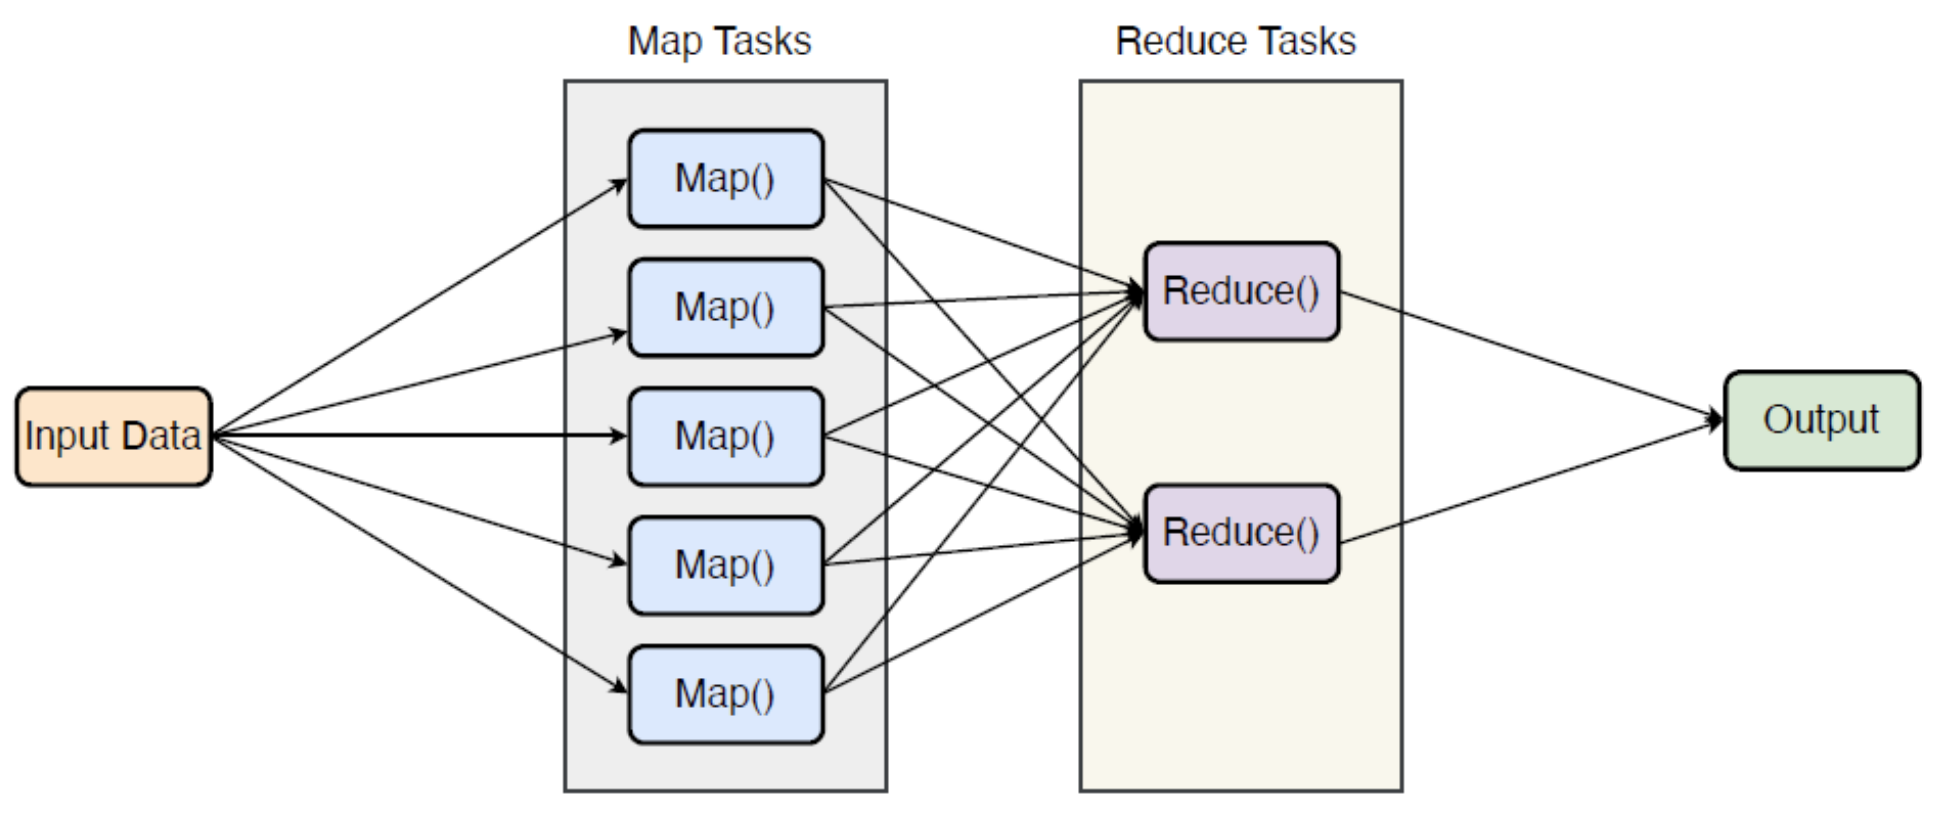
\includegraphics[width=0.75\textwidth]{media/arch.png}
		\caption{MapReduce overall architecture and execution pipeline.}
		\label{fig:project_overview}
	\end{figure}
	
	\section{Dataset Analysis and Preprocessing}
	We utilize the Amazon Reviews Dataset compiled in 2023 by McAuley Lab, which includes over 571 million reviews globally. To match local computational parameters, we isolated the \textbf{Software} category subset. 
	
	\subsection{Data Schema}
	The raw dataset is stored in standard JSON-Lines (\texttt{.jsonl}) format. Each JSON record represents an individual review containing the schema detailed in Table 1.
	
	\begin{table}[htbp]
		\centering
		\caption{Software Review Dataset Schema details.}
		\begin{tabular}{lp{3.5cm}p{7cm}}
			\toprule
			\textbf{Field} & \textbf{Type} & \textbf{Explanation} \\
			\midrule
			\texttt{rating} & float & Product score given by consumer (ranging from 1.0 to 5.0) \\
			\texttt{title} & string & Textual headline summary of the review \\
			\texttt{text} & string & Primary body paragraph of the review \\
			\texttt{asin} & string & Unique Amazon Standard Identification Number (Product ID) \\
			\texttt{parent\_asin} & string & Parent identification number for grouping product variations \\
			\texttt{user\_id} & string & Unique identification key for the reviewer \\
			\texttt{timestamp} & integer & Epoch Unix timestamp when the review was generated \\
			\texttt{verified\_purchase} & boolean & Verification indicator if purchase was completed on Amazon \\
			\texttt{helpful\_vote} & integer & Number of positive feedback votes identifying review quality \\
			\bottomrule
		\end{tabular}
	\end{table}
	
	\subsection{Preprocessing Pipeline}
	A specialized Python dataset analysis tool (\texttt{dataset.py}) was built to read the raw files, count basic elements, handle null records, and a Jupyter notebook that would write the consolidated dataset into a clean runtime file at \texttt{data/software-clean.jsonl}. This step removed corrupt JSON items, ensuring downstream MapReduce code runs without interruption such as division by zero.
	
	\section{Tasks}
	
	In this section, we present the methodology, python scripts, and output patterns for each of our analytical pipelines.
	
	\subsection{Task 1: Counting reviews per product}
	\paragraph{} 
	To determine the frequency of user interactions per product, we mapped each record using the \texttt{asin} key. The mapper emits a pair of $(\text{asin}, 1)$ for every valid review. The MapReduce shuffle-and-sort phase routes all occurrences of an \texttt{asin} to the same reducer, which performs a summation of values to deliver the total volume.
	
	\paragraph{Python Code Snippet (\texttt{reviews.py}):}
	\begin{lstlisting}[language=Python, caption={MapReduce program to count reviews per product.}]
from mrjob.job import MRJob
import json

class MRReviewsCount(MRJob):

	def mapper(self, _, line):
		try:
			review = json.loads(line)
			asin = review.get('asin')
			if asin:
				yield asin, 1
		except json.JSONDecodeError:
			pass
	
	def reducer(self, key, values):
		yield key, sum(values)
	
if __name__ == "__main__":
	MRReviewsCount.run()
	\end{lstlisting}
	
	\paragraph{Output (clipped sample):}
	\begin{verbatim}
		"B00004Y7D4"  24
		"B000051S8K"  5
		"B0000531AF"  112
	\end{verbatim}

	
	\subsection{Task 2: Computing average star rating per product}
	\paragraph{} 
	The rating distribution is calculated by capturing the real number ratings corresponding to each item. The mapper extracts the product ID (\texttt{asin}) and the corresponding numerical value \texttt{rating}, yielding $(\text{asin}, \text{rating})$. In the reducer, the aggregated values are cast to a list, aggregated via summation, and divided by the element count.
	$$\text{Average Rating} = \frac{\sum_{i=1}^{N} \text{rating}_i}{N}$$
	
	\paragraph{Python Code Snippet (\texttt{average\_rating.py}):}
	\begin{lstlisting}[language=Python, caption={MapReduce job to calculate average star ratings.}]
from mrjob.job import MRJob
import json

class MRAverageRating(MRJob):

	def mapper(self, _, line):
		try:
			review = json.loads(line)
			asin = review['asin']
			rating = review['rating']
			yield asin, rating
		
		except:
			pass
		
	def reducer(self, key, values):
		ratings = list(values)
		total = sum(ratings)
		count = len(ratings)
	
		if count > 0:
		yield key, total / count
	
if __name__ == "__main__":
	MRAverageRating.run()
	\end{lstlisting}
	
	
	\subsection{Task 3: Identifying top ten most reviewed products}
	\paragraph{} 
	Finding a global Top-10 list requires a multi-step MapReduce program because a simple reducer only aggregates values locally per key. 
	In Step 1, the mapper yields $(\text{asin}, 1)$ and the reducer yields $(\text{None}, (\text{asin}, \sum 1))$. This structures all results under a single virtual key (\texttt{None}).
	In Step 2, a single reducer receives this combined list, sorts them in descending order by review count, and returns the first 10 items.
	
	\paragraph{Python Code Snippet (\texttt{top\_ten.py}):}
	\begin{lstlisting}[language=Python, caption={Multi-step  job to isolate top ten reviewed items.}]
from mrjob.job import MRJob
import json
from mrjob.step import MRStep

class MRTop10Products(MRJob):

	def mapper(self, _, line):
		try:
			review = json.loads(line)
			asin = review.get('asin')
			if asin:
				yield asin, 1
		except json.JSONDecodeError:
			pass
	
	def reducer(self, asin, values):
		yield None, (asin, sum(values))
	
	def reduceTopTen(self, _, values):
		top = sorted(values, reverse=True)[:10]
		for asin, count in top:
		yield asin, count
	
	def steps(self):
		return [
			MRStep(mapper=self.mapper, reducer=self.reducer),
			MRStep(reducer=self.reduceTopTen)       
		]
	
if __name__ == "__main__":
	MRTop10Products.run()
	\end{lstlisting}

	
	\subsection{Task 4: Evaluating Helpful vote ratios}
	\paragraph{} 
	We process helpfulness by classifying reviews into binary buckets. The mapper examines the \texttt{helpful\_vote} field; if the value is $0$, it yields $(\text{"unhelpful"}, 1)$, otherwise it yields $(\text{"helpful"}, 1)$. 
	Using a secondary reduction step, the global ratio is evaluated:
	$$\text{Average Helpfulness Score} = \frac{\text{Helpful Votes}}{\text{Helpful} + \text{Unhelpful Votes}}$$
	
	\paragraph{Python Code Snippet (\texttt{helpfulness.py}):}
	\begin{lstlisting}[language=Python, caption={Evaluating customer helpfulness ratios using multi-step execution.}]
		from mrjob.job import MRJob
		import json
		from mrjob.step import MRStep
		
		class MRHelpfulness(MRJob):
		
			def mapper(self, _, line):
				try:
					review = json.loads(line)
					vote = review.get('helpful_vote')
					if vote == 0:
						yield 'unhelpful', 1
					else:
						yield 'helpful', 1
				except json.JSONDecodeError:
					pass
			
			def reducer(self, vote, values):
				yield None, (vote, sum(values))
			
			def reducerAvg(self, _, values):
				helpful = 0
				unhelpful = 0
				
				for vote, count in values:
					if vote == "helpful":
						helpful = count
					else:
						unhelpful = count
				
				total = helpful + unhelpful
				avg = helpful / total if total > 0 else 0
				
				yield "ave_helpful_score", avg
			
			def steps(self):
				return [
					MRStep(mapper=self.mapper, reducer=self.reducer),
					MRStep(reducer=self.reducerAvg)       
				]
			
		if __name__ == "__main__":
			MRHelpfulness.run()
	\end{lstlisting}
	

	\subsection{Task 5: Text Sentiment Analysis}
	\paragraph{} 
	To assess user satisfaction, we performed text-based Sentiment Analysis. In the mapper class, we initialized the NLTK \texttt{SentimentIntensityAnalyzer} (VADER). It parses raw text data and computes a compound metric score ranging between $-1$ and $+1$. 
	\begin{itemize}
		\item \textbf{Positive Sentiment:} $\text{Score} \geq 0.05$
		\item \textbf{Negative Sentiment:} $\text{Score} \leq -0.05$
		\item \textbf{Neutral Sentiment:} $-0.05 < \text{Score} < 0.05$
	\end{itemize}
	The reducer aggregates the frequency counters across the three distinct sentiments.
	
	\paragraph{Python Code Snippet (\texttt{sentiment.py}):}
	\begin{lstlisting}[language=Python, caption={Distributed sentiment evaluation of review text using VADER NLP.}]
		from mrjob.job import MRJob
		from nltk.sentiment import SentimentIntensityAnalyzer
		import json
		
		class MRSentimentAnalysis(MRJob):
		
			def mapper_init(self):
				self.analyzer = SentimentIntensityAnalyzer()
			
			def mapper(self, _, line):
				try:
					review = json.loads(line)
					text = review.get("text", "")
				
					if text:
						score = self.analyzer.polarity_scores(text)["compound"]
				
					if score >= 0.05:
						yield "positive", 1
					elif score <= -0.05:
						yield "negative", 1
					else:
						yield "neutral", 1
				except Exception:
					pass
			
			def reducer(self, sentiment, counts):
				yield sentiment, sum(counts)
			
		if __name__ == "__main__":
			MRSentimentAnalysis.run()
	\end{lstlisting}
	
	\newpage
	
	\section{Analysis of Results}
	We collected the output values of our MapReduce processes, converted them to structured format (CSV), and evaluated them through a jupyter notebook using \texttt{matplotlib} and \texttt{pandas}.
	
	\subsection{Product Ratings Distribution}
	The rating system demonstrates extreme behavior. Most products gather scores concentrated closely around the extremes ($1.0$ and $5.0$). 
	This dual-peak outcome is typical in retail reviews: extremely happy customers write reviews, as do highly frustrated customers, whereas moderately satisfied buyers rarely write reviews.
	
	\begin{figure}[H]
		\centering
		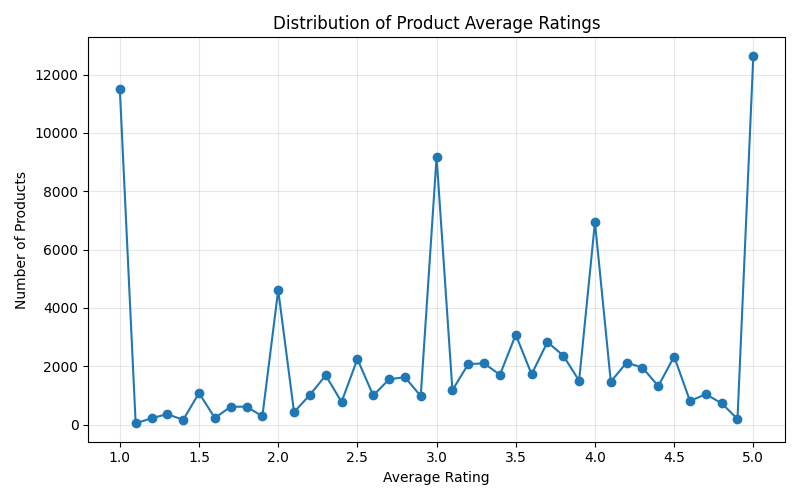
\includegraphics[width=0.75\textwidth]{media/avg-rating-distribution.png}
		\caption{Empirical distribution of average product ratings demonstrating dual-peak clustering.}
		\label{fig:rating_dist}
	\end{figure}
	
	\subsection{Sentiment Classification Analysis}
	We compiled the sentiment analysis classifications from all records giving: 
	
	\begin{figure}[H]
		\centering
		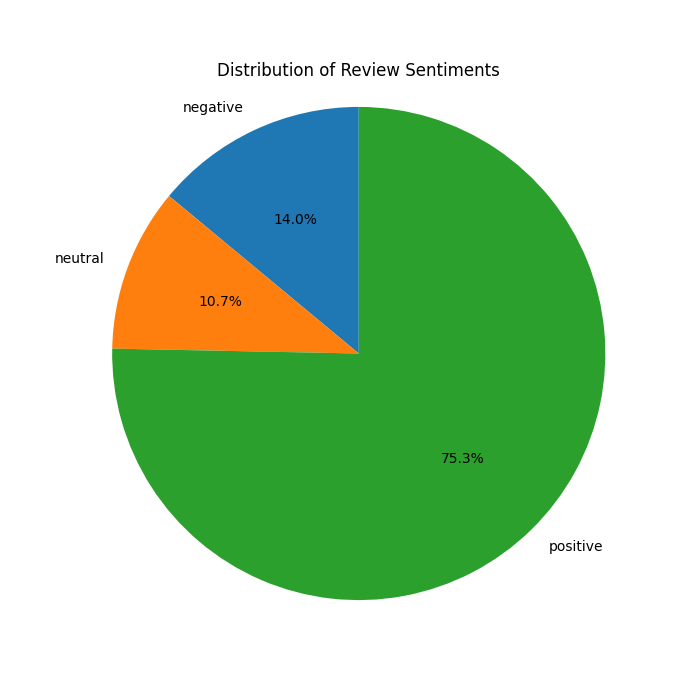
\includegraphics[width=0.5\textwidth]{media/pie-sentiment.png}
		\caption{Review classifications into Positive, Neutral, and Negative segments.}
		\label{fig:pie_sentiment}
	\end{figure}
	
	The distribution of review sentiments across the dataset is categorized as follows:
	\begin{itemize}
		\item \textbf{Positive =} 75.3\%
		\item \textbf{Negative =} 14.0\%
		\item \textbf{Neutral =} 10.7\%
	\end{itemize}
	
	This heavily right-skewed positive presence indicates that users are overall highly satisfied with software products, or that positive language is naturally dominant in verified customer experiences.
	
	\begin{figure}[H]
		\centering
		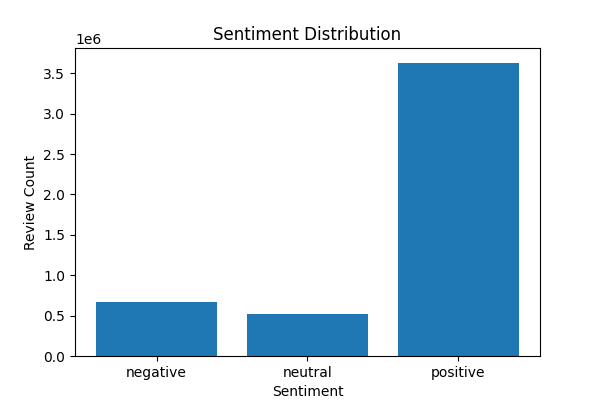
\includegraphics[width=0.75\textwidth]{media/sentiment-distribution.png}
		\caption{Absolute volume count of sentiment records across the software category.}
		\label{fig:bar_sentiment}
	\end{figure}
	
	\section{Conclusion}
	This project successfully implemented a series of distributed MapReduce analytical tasks to query, aggregate, and process customer reviews in the Amazon Software category. By leveraging the \texttt{mrjob} framework, we demonstrated how high-volume sentiment classification, ranking, and statistical calculations can be split into local parallel execution units.
	
	Future additions to this workflow could include:
	\begin{enumerate}
		\item \textbf{Deployment to AWS EMR:} Porting this localized implementation directly onto a live Hadoop/Spark architecture in Amazon Elastic MapReduce to process the complete 571-million review archive.
		\item \textbf{Advanced NLP Modeling:} Upgrading basic VADER lexical rules to heavier contextual embedding classifiers, such as DistilBERT, during Map phases.
		\item \textbf{Item-to-Item Collaborative Filtering:} Expanding basic metric counts into multi-pass jobs calculating co-occurrence vectors to build an active recommendation service.
	\end{enumerate}
	
	\section*{References}
	\begin{enumerate}
		\item McAuley, J., et al. \textit{Amazon Reviews 2023 Dataset.} \url{https://amazon-reviews-2023.github.io/}
		\item Dean, J., \& Ghemawat, S. (2008). \textit{MapReduce: Simplified Data Processing on Large Clusters.} ACM Communications. \url{https://static.googleusercontent.com/media/research.google.com/es/us/archive/mapreduce-osdi04.pdf}
		\item Python \texttt{mrjob} Library Documentation. \url{https://mrjob.readthedocs.io/}
		\item NLTK Sentiment Intensity Analyzer Documentation. \url{https://www.nltk.org/api/nltk.sentiment.SentimentIntensityAnalyzer.html}
	\end{enumerate}
	
\end{document}